%% abtex2-modelo-relatorio-tecnico.tex, v<VERSION> laurocesar
%% Copyright 2012-2015 by abnTeX2 group at http://abntex2.googlecode.com/ 
%%
%% This work may be distributed and/or modified under the
%% conditions of the LaTeX Project Public License, either version 1.3
%% of this license or (at your option) any later version.
%% The latest version of this license is in
%%   http://www.latex-project.org/lppl.txt
%% and version 1.3 or later is part of all distributions of LaTeX
%% version 2005/12/01 or later.
%%
%% This work has the LPPL maintenance status `maintained'.
%% 
%% The Current Maintainer of this work is the abnTeX2 team, led
%% by Lauro César Araujo. Further information are available on 
%% http://abntex2.googlecode.com/
%%
%% This work consists of the files abntex2-modelo-relatorio-tecnico.tex,
%% abntex2-modelo-include-comandos and abntex2-modelo-references.bib
%%

% ------------------------------------------------------------------------
% ------------------------------------------------------------------------
% abnTeX2: Modelo de Relatório Técnico/Acadêmico em conformidade com 
% ABNT NBR 10719:2011 Informação e documentação - Relatório técnico e/ou
% científico - Apresentação
% ------------------------------------------------------------------------ 
% ------------------------------------------------------------------------

\documentclass[
	% -- opções da classe memoir --
	12pt,				% tamanho da fonte
	openright,			% capítulos começam em pág ímpar (insere página vazia caso preciso)
	oneside,			% para impressão em verso e anverso. Oposto a oneside
	a4paper,			% tamanho do papel. 
	% -- opções da classe abntex2 --
	%chapter=TITLE,		% títulos de capítulos convertidos em letras maiúsculas
	%section=TITLE,		% títulos de seções convertidos em letras maiúsculas
	%subsection=TITLE,	% títulos de subseções convertidos em letras maiúsculas
	%subsubsection=TITLE,% títulos de subsubseções convertidos em letras maiúsculas
	% -- opções do pacote babel --
	english,			% idioma adicional para hifenização
	french,				% idioma adicional para hifenização
	spanish,			% idioma adicional para hifenização
	brazil,				% o último idioma é o principal do documento
	]{abntex2}

% ---
% PACOTES
% ---
% Pacotes fundamentais 
% ---
\usepackage{lmodern}			% Usa a fonte Latin Modern
\usepackage[T1]{fontenc}		% Selecao de codigos de fonte.
\usepackage[utf8]{inputenc}		% Codificacao do documento (conversão automática dos acentos)
\usepackage{indentfirst}		% Indenta o primeiro parágrafo de cada seção.
\usepackage{color}				% Controle das cores
\usepackage{graphicx}			% Inclusão de gráficos
\usepackage{microtype} 			% para melhorias de justificação
\usepackage{lastpage}
\usepackage{pdflscape} 			% páginas em modo paisagem

% ---

% ---
% Pacotes adicionais para glossário
% ---
\usepackage[noredefwarn,acronym,toc,subentrycounter,seeautonumberlist,sort=standard]{glossaries}
\usepackage{xparse}             % For dualentry glossary + acronym personalized command

% ---
% Pacotes adicionais, usados no anexo do modelo de folha de identificação
% ---
\usepackage{multicol}
\usepackage{multirow}
% ---
	
% ---
% Pacotes adicionais, usados apenas no âmbito do Modelo Canônico do abnteX2
% ---
%\usepackage{lipsum}				% para geração de dummy text
% ---

% ---
% Pacotes de citações
% ---
\usepackage[brazilian,hyperpageref]{backref}	 % Paginas com as citações na bibl
\usepackage[alf]{abntex2cite}	% Citações padrão ABNT

% ---
% Alterando altura do cabeçalho
\usepackage{salmj}
\usepackage{listings}

% ---
% Pacotes para desenhos
\usepackage{tikz}
\usetikzlibrary{shapes,arrows}
\usepackage{pgfplots}
% --- 
% CONFIGURAÇÕES DE PACOTES
% --- 

% ---
% Configurações do pacote backref
% Usado sem a opção hyperpageref de backref
\renewcommand{\backrefpagesname}{Citado na(s) página(s):~}
% Texto padrão antes do número das páginas
\renewcommand{\backref}{}
% Define os textos da citação
\renewcommand*{\backrefalt}[4]{
	\ifcase #1 %
		Nenhuma citação no texto.%
	\or
		Citado na página #2.%
	\else
		Citado #1 vezes nas páginas #2.%
	\fi}%
% ---

% Altera o nome padrão do rótulo usado no comando \autoref{}
\renewcommand{\lstlistingname}{Código}

% Altera o rótulo a ser usando no elemento pré-textual "Lista de código"
\renewcommand{\lstlistlistingname}{Lista de códigos}

% Configura a ``Lista de Códigos'' conforme as regras da ABNT (para abnTeX2)
\begingroup\makeatletter
\let\newcounter\@gobble\let\setcounter\@gobbletwo
  \globaldefs\@ne \let\c@loldepth\@ne
  \newlistof{listings}{lol}{\lstlistlistingname}
  \newlistentry{lstlisting}{lol}{0}
\endgroup

\renewcommand{\cftlstlistingaftersnum}{\hfill--\hfill}

\let\oldlstlistoflistings\lstlistoflistings
\renewcommand{\lstlistoflistings}{%
   \begingroup%
   \let\oldnumberline\numberline%
   \renewcommand{\numberline}{\lstlistingname\space\oldnumberline}%
   \oldlstlistoflistings%
   \endgroup}


\definecolor{mygreen}{rgb}{0,0.6,0}
\definecolor{mygray}{rgb}{0.5,0.5,0.5}
\definecolor{mymauve}{rgb}{0.58,0,0.82}

\lstset{ %
  backgroundcolor=\color{white},   % choose the background color; you must add \usepackage{color} or \usepackage{xcolor}
  basicstyle=\footnotesize,        % the size of the fonts that are used for the code
  breakatwhitespace=false,         % sets if automatic breaks should only happen at whitespace
  breaklines=true,                 % sets automatic line breaking
  captionpos=b,                    % sets the caption-position to bottom
  commentstyle=\color{mygreen},    % comment style
  deletekeywords={...},            % if you want to delete keywords from the given language
  escapeinside={\%*}{*)},          % if you want to add LaTeX within your code
  extendedchars=true,              % lets you use non-ASCII characters; for 8-bits encodings only, does not work with UTF-8
  frame=single,                    % adds a frame around the code
  keepspaces=true,                 % keeps spaces in text, useful for keeping indentation of code (possibly needs columns=flexible)
  keywordstyle=\color{blue},       % keyword style
  language=Octave,                 % the language of the code
  otherkeywords={*,...},            % if you want to add more keywords to the set
  numbers=left,                    % where to put the line-numbers; possible values are (none, left, right)
  numbersep=5pt,                   % how far the line-numbers are from the code
  numberstyle=\tiny\color{mygray}, % the style that is used for the line-numbers
  rulecolor=\color{black},         % if not set, the frame-color may be changed on line-breaks within not-black text (e.g. comments (green here))
  showspaces=false,                % show spaces everywhere adding particular underscores; it overrides 'showstringspaces'
  showstringspaces=false,          % underline spaces within strings only
  showtabs=false,                  % show tabs within strings adding particular underscores
  stepnumber=2,                    % the step between two line-numbers. If it's 1, each line will be numbered
  stringstyle=\color{mymauve},     % string literal style
  tabsize=2,                       % sets default tabsize to 2 spaces
  title=\lstname                   % show the filename of files included with \lstinputlisting; also try caption instead of title
}   
   
   
   
%%%%%% Configurações do pacote Tikz para diagramas
\tikzstyle{block} = [rectangle, draw, fill=blue!20, 
    text width=5em, text centered, rounded corners, minimum height=4em]
\tikzstyle{line} = [draw, -latex']
%\newcommand{\imprimeNumeroContrato}{}
%\newcommand{\imprimeValorProduto}{}
%\newcommand{\imprimeValorContrato}{}
%\newcommand{\imprimeDataEntrega}{}
%\newcommand{\imprimeLabelSupervisor}{}
%\newcommand{\imprimeSupervisor}{}
%\newcommand{\numeroContrato}[1]{\renewcommand{\imprimeNumeroContrato}{#1}}
%\newcommand{\valorProduto}[1]{\renewcommand{\imprimeValorProduto}{#1}}
%\newcommand{\valorContrato}[1]{\renewcommand{\imprimeValorContrato}{#1}}
%\newcommand{\dataEntrega}[1]{\renewcommand{\imprimeDataEntrega}{#1}}
%\newcommand{\supervisor}[2][Nome do supervisor]{%
%\renewcommand{\imprimeLabelSupervisor}{#1}%
%\renewcommand{\imprimeSupervisor}{#2}%
%}
\setheadfoot{78.5pt}{12.2pt}
\setlength\headsep{0.6\headsep}
\setlength\textheight{0.92\textheight}

%Needs xparse package - Dual Entry for glossary (glossary + acronym)
\DeclareDocumentCommand{\newdualentry}{ O{} O{} m m m m } {
  \newglossaryentry{gls-#3}{name={#5},text={#5\glsadd{#3}},
    description={#6},sort={#3}
  }
  \newacronym[see={[Glossário: ]{gls-#3}},#2]{#3}{#4}{#5\glsadd{gls-#3}}
}
% ---
% Informações de dados para CAPA e FOLHA DE ROSTO
% ---
\titulo{Produto 4 - Relatório contendo requisitos técnicos para desenvolvimento de software, na forma de aplicativo móvel, para viabilizar ferramentas de participação social para dispositivos móveis.}
\autor{Diego Rabatone Oliveira}
\local{Brasil}
\data{Junho/2015, v1}
\newcommand{\numeroContrato}{2015/000042-00}
\newcommand{\valorProduto}{R\$9.800,00 (nove mil e oitocentos reais)}
\newcommand{\valorContrato}{R\$40.000,00 (quarenta mil reais}
\newcommand{\dataEntrega}{15/06/2015}
\newcommand{\labelSupervisor}{Supervisora}
\newcommand{\supervisor}{Sabrina Durigon Marques}
\instituicao{%
  Secretaria de Assuntos Legislativos do 
  \par
  Ministério da Justiça (SAL/MJ)}
\orientador[Supervisora:]{Sabrina Durigon Marques}

\tipotrabalho{Relatório técnico}
% O preambulo deve conter o tipo do trabalho, o objetivo, 
% o nome da instituição e a área de concentração 
\preambulo{Relatório referente ao Projeto BRA/07/004 – Democratização de Informações no Processo de Elaboração Normativa}
% ---

% ---
% Configurações de aparência do PDF final

% alterando o aspecto da cor azul
\definecolor{blue}{RGB}{41,5,195}

% informações do PDF
\makeatletter
\hypersetup{
     	%pagebackref=true,
		pdftitle={\@title}, 
		pdfauthor={\@author},
    	pdfsubject={\imprimirpreambulo},
	    pdfcreator={LaTeX with abnTeX2},
		pdfkeywords={Pensando O Direito}{Ministério da Justiça}{Aplicativo Móvel}{Participação Social}, 
		colorlinks=true,       		% false: boxed links; true: colored links
    	linkcolor=blue,          	% color of internal links
    	citecolor=blue,        		% color of links to bibliography
    	filecolor=magenta,      		% color of file links
		urlcolor=blue,
		bookmarksdepth=4
}
\makeatother
% --- 
%\begin{siglas}
%  \item[ABNT] Associação Brasileira de Normas Técnicas
%  \item[abnTeX] ABsurdas Normas para TeX
%\end{siglas}

%\newacronym%
%[description={}]%
%{}{}{}%

%\hyphenation{Django}%
%\newglossaryentry{django}{%
%    name=Django,%
%    description={\'{e} um framework para desenvolvimento r\'{a}pido para web, escrito em %Python, que utiliza o padr\~{a}o MVT}%
%}%
%\newdualentry{mvc}{MVC}{\textit{Model View Controller}}{\textit{Design Pattern} muito conhecida e introduzida por \textit{Erich Gamma} em 1995}
%\newacronym{html}{HTML}{HyperText Markup Language}

\newacronym{sal}{SAL/MJ}{Secretaria de Assuntos Legislativos do Ministério da Justiça}
\newacronym{pnud}{PNUD}{Programa das Nações Unidas para o Desenvolvimento}
\newcommand{\mc}{Marco Civil da Internet}
\newcommand{\pdp}{Proteção de Dados Pessoais}

\glsresetall
% ---
% compila o indice
\makeindex

% ----
% Início do documento
\begin{document}
\pagestyle{estilosalmj}
\aliaspagestyle{chapter}{estilosalmj}% customizing chapter pagestyle

% Seleciona o idioma do documento (conforme pacotes do babel)
%\selectlanguage{english}
\selectlanguage{brazil}

% Retira espaço extra obsoleto entre as frases.
\frenchspacing 

% ----------------------------------------------------------
% ELEMENTOS PRÉ-TEXTUAIS

% ---
% Capa
\imprimircapa

% ---
% Folha de rosto
% (o * indica que haverá a ficha bibliográfica)
\imprimirfolhaderosto*

% ---
% Anverso da folha de rosto:

{
\ABNTEXchapterfont

\begin{fichacatalografica}
	\sffamily
	\vspace*{\fill}					% Posição vertical
	\begin{center}					% Minipage Centralizado
	\fbox{\begin{minipage}[c][8cm]{13.5cm}		% Largura
	\small
	\imprimirautor
	%Sobrenome, Nome do autor
	
	\hspace{0.5cm} \imprimirtitulo  / \imprimirautor. --
	\imprimirlocal, \imprimirdata-
	
	\hspace{0.5cm} \pageref{LastPage} p. : il. (algumas color.) ; 30 cm.\\
	
	\hspace{0.5cm} \imprimirorientadorRotulo~\imprimirorientador\\
	
	\hspace{0.5cm}
	\parbox[t]{\textwidth}{\imprimirtipotrabalho~--~\imprimirinstituicao,
	\imprimirdata.}\\
	
	\hspace{0.5cm}
		1. Redes Sociais.
		2. Relatório.
		I. Sabrina Durigon Marques.
		II. Secretaria de Assuntos Legislativos.
		III. Ministério da Justiça.
		IV. \imprimirtitulo
	\end{minipage}}	
	\end{center}

	\footnotesize{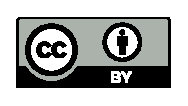
\includegraphics[scale=0.5]{./imagens/ccby.eps} Este trabalho está licenciado com uma Licença \href{http://creativecommons.org/licenses/by/4.0/}{Creative Commons - Atribuição 4.0 Internacional}.}
\end{fichacatalografica}

}

% ---
% Agradecimentos
%\begin{agradecimentos}
%O agradecimento principal é direcionado a Youssef Cherem, autor do
%\nameref{formulado-identificacao} (\autopageref{formulado-identificacao}).
%
%Os agradecimentos especiais são direcionados ao Centro de Pesquisa em
%Arquitetura da Informação\footnote{\url{http://www.cpai.unb.br/}} da Universidade de
%Brasília (CPAI), ao grupo de usuários
%\emph{latex-br}\footnote{\url{http://groups.google.com/group/latex-br}} e aos
%novos voluntários do grupo
%\emph{\abnTeX}\footnote{\url{http://groups.google.com/group/abntex2} e
%\url{http://abntex2.googlecode.com/}}~que contribuíram e que ainda
%contribuirão para a evolução do abn\TeX.
%
%\end{agradecimentos}
% ---


% ---
% RESUMO
% resumo na língua vernácula (obrigatório)
\setlength{\absparsep}{18pt} % ajusta o espaçamento dos parágrafos do resumo
\begin{resumo}
Este produto objetiva primeiramente a proposição de soluções para geração de relatório agregado que organize e consolide as contribuições recebdidas pelas ferramentas e aplicações de consulta pública. Além disso, também será complementada a proposta de organização das atividades de desenvolvimento, considerando a utilização de métodos ágeis.

 \noindent
 \textbf{Palavras-chaves}: consolidação, relatório, organização, Métodos Ágeis.
\end{resumo}
% ---

% ---
% inserir lista de símbolos
%\begin{simbolos}
%  \item[$ \Gamma $] Letra grega Gama
%  \item[$ \Lambda $] Lambda
%  \item[$ \zeta $] Letra grega minúscula zeta
%  \item[$ \in $] Pertence
%\end{simbolos}


% ---
% inserir o sumario
% ---
\pdfbookmark[0]{\contentsname}{toc}
\tableofcontents*
\cleardoublepage
% ---


% ----------------------------------------------------------
% ELEMENTOS TEXTUAIS
% ----------------------------------------------------------
\textual
\pagestyle{estilosalmj}
\aliaspagestyle{chapter}{estilosalmj}% customizing chapter pagestyle

% ---
% Introdução
%------
%Se deseja-se o capítulo listado no índice mas que apareça aqui sem numeração.
%--
%\chapter*[Introdução]{Introdução}
%\addcontentsline{toc}{chapter}{Introdução}
%------
\chapter{Introdução}


\section{Objetivo}


% ---
% Desenvolvimento
\chapter{Desenvolvimento}
No sentido de melhorar a inserção do projeto Pensando o Direito e correlatos, 
abaixo estão descritas algumas iniciativas que visam uma maior integração em
termos de processos de comunicação e outras que podem ajudar a embasar futuros
estudos e iniciativas.

\section{Redes Sociais privadas}
De acordo com \citeonline{serasa}, em novembro de 2014 o Facebook ocupava a primeira posição no ranking das redes sociais mais visitadas do Brasil com 64,82\% de participação. Em seguida temos o Youtube, com 26,04\%, e, em quarto lugar, o Twitter, com 1,36\% do mercado. Na Figura \ref{fig:social-network-share-br} podemos observar as 10 primeiras redes sociais:
\begin{figure}[htb]%
	\begin{center}
		\begin{tikzpicture}
		  \begin{axis}[
		    xbar, xmin=0, xmax=75,
		    %grid=major,
		    width=12cm, height=11cm, enlarge y limits=0.1,
		    xlabel={\% de participação},
		    symbolic y coords={LinkedIn,{Bate Papo UOL},Badoo,{Haboo Brasil},Instagram,Google+,Twitter,{Yahoo! Answers Brasil},Youtube,Facebook},
		    ytick=data,
		   	legend style={at={(0.2,-0.07)}, anchor=north,legend columns=-1},
		    nodes near coords, nodes near coords align={horizontal},
		    ]
		    \addplot
			[draw=blue, pattern=horizontal lines light blue]
		    coordinates {(0.35,{Bate Papo UOL}) (0.36,Badoo) (0.47,{Haboo Brasil}) (0.54,Instagram) (0.70,Google+) (1.36,Twitter) (1.47,{Yahoo! Answers Brasil}) (26.04,Youtube) (64.82,Facebook) (0.30,LinkedIn) };
			\legend{Brasil}
		  \end{axis}
		\end{tikzpicture}
    	%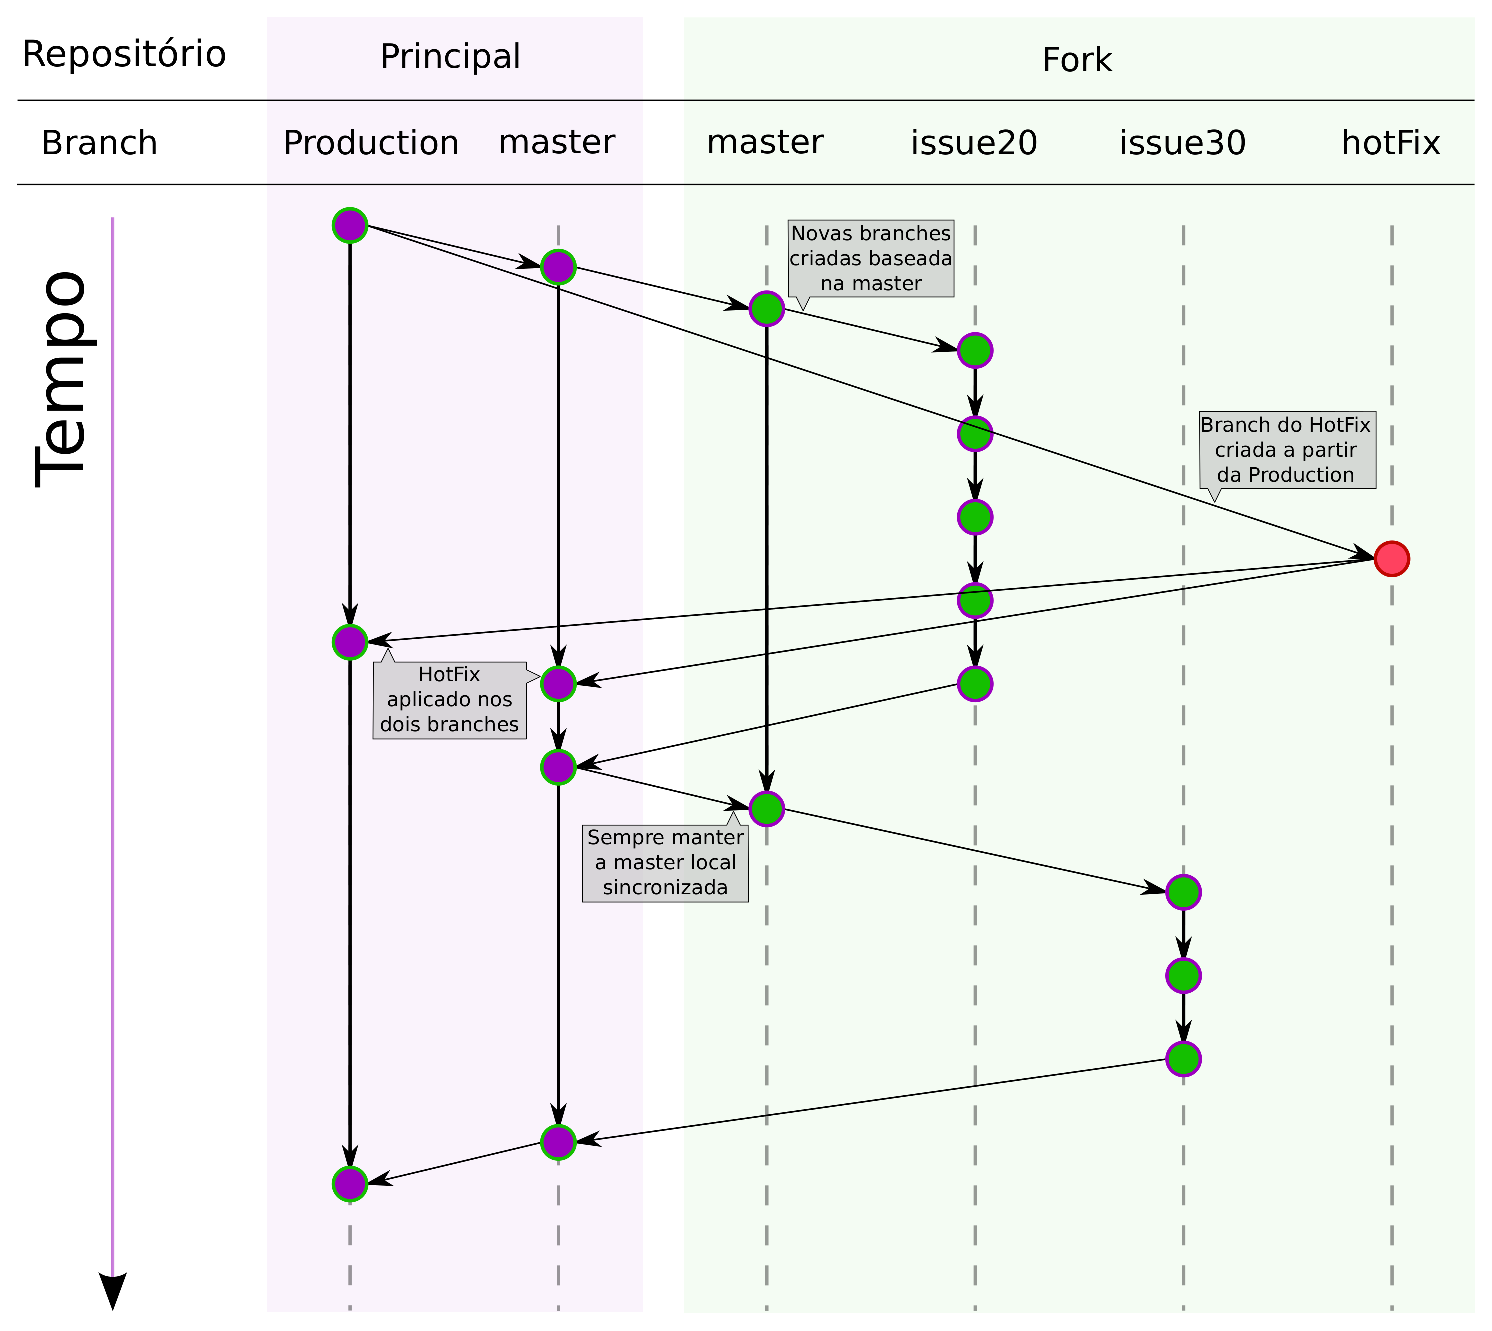
\includegraphics[scale=0.65]{./imagens/branchForkDiagram.eps}%
	\end{center}%
	\caption{10 maiores redes sociais em número de acessos no Brasil em novembro de 2104\label{fig:social-network-share-br}}%
	\fonte{Autoria Própria, baseado em \citeonline{serasa}}%
\end{figure}%

Na Figura \ref{fig:social-network-pensando} observamos as estatísticas de acesso, originados nas redes sociais, do projeto Pensando o Direito e das consultas públicas, com destaque especial para o Facebook com 90,91\% e para o Twitter com 7,1\%.
\begin{figure}[htb]%
	\begin{center}
		\begin{tikzpicture}
		  \begin{axis}[
		    xbar, xmin=0, xmax=105,
		    %grid=major,
		    width=12cm, height=12cm, enlarge y limits=0.1,
		    xlabel={\% de participação},
		    symbolic y coords={
			    {paper.li},
			    reddit,
			    Disqus,
			    {goo.gl},
			    Pocket,
			    LinkedIn,
			    Blogger,
			    Google+,
			    Twitter,
			    Facebook
		    },
		    ytick=data,
		    yticklabel style={/pgf/number format/fixed},
		    legend style={at={(0.12,-0.06)}, anchor=north,legend columns=-1},
		    nodes near coords, nodes near coords align={horizontal},
		    ]
		    %Pensando o Direito
		    \addplot
			[draw=black,pattern=horizontal lines dark blue]
		    coordinates {
			    (0.01,{paper.li})
			    (0.06,reddit)
			    (0.06,Disqus)
			    (0.13,{goo.gl})
			    (0.16,Pocket)
			    (0.18,LinkedIn)
			    (0.48,Blogger)
			    (0.9,Google+)
			    (7.10,Twitter)
			    (90.91,Facebook)
		    };
		  	\legend{Pensando}
		  \end{axis}
		\end{tikzpicture}
	\end{center}%
	\caption{10 redes sociais que mais direcionam acessos à plataforma Pensando O Direito\label{fig:social-network-pensando}}%
	\fonte{Autoria Própria baseado em estatísticas do Google Analytics}%
\end{figure}%

Na Figura \ref{fig:social-network-pensando-e-mercado} podemos observar a comparação entre as estatísticas de cotas do mercado brasileiro e as estatísticas do projeto Pensando o Direito. Como pode-se observar, o Facebook possui uma predominância muito maior no projeto Pensando O Direito (90,91\%) do que no mercado (64,82\%), assim como o Twitter (7,1\% no Pensando O Direito \textit{versus} 1,36\% no mercado).

Por outro lado, o Youtube sequer aparece nas estatísticas de origem de acesso do projeto Pensando O Direito, apesar de ser a segunda rede social mais acessada no Brasil com 26,04\% do mercado. Daqui percebe-se que um ponto importante a ser melhorado na comunicação do projeto Pensando O Direito seria trabalhar melhor a divulgação no YouTube. Para tanto, recomenda-se uma nova linha de ação na comunicação focada no Youtube. Neste sentido, seria importante que todos os projetos ligados ao Pensando O Direito sejam concentrados numa única conta, e também é fundamental que na descrição de todos os vídeos existam links que remetam a páginas do projeto, ou de alguma consulta pública, ligadas ao vídeo.

\begin{figure}[htb]%
	\begin{center}
		\begin{tikzpicture}
		  \begin{axis}[
		    xbar, xmin=0, xmax=105,
		    %grid=major,
		    width=12cm, height=14cm, enlarge y limits=0.1,
		    xlabel={\% de participação},
		    symbolic y coords={LinkedIn,{Bate Papo UOL},Badoo,{Haboo Brasil},Instagram,Google+,Twitter,{Yahoo! Answers Brasil},Youtube,Facebook},
		    ytick=data,
		    legend style={at={(0.12,-0.05)}, anchor=north,legend columns=-1}, 
		    nodes near coords, nodes near coords align={horizontal},
		    ]
		    %Brasil
		    \addplot
			[draw=blue, pattern=horizontal lines light blue]
		    coordinates {
		    	(0.35,{Bate Papo UOL})
		    	(0.36,Badoo)
		    	(0.47,{Haboo Brasil})
		    	(0.54,Instagram)
		    	(0.70,Google+)
		    	(1.36,Twitter)
		    	(1.47,{Yahoo! Answers Brasil})
		    	(26.04,Youtube)
		    	(64.82,Facebook)
		    	(0.30,LinkedIn)
		    };
		    %Pensando o Direito
		    \addplot
			[draw=black,pattern=horizontal lines dark blue]
		    coordinates {
		    	(0,{Bate Papo UOL})
		    	(0,Badoo)
		    	(0,{Haboo Brasil})
		    	(0,Instagram)
		    	(0.90,Google+)
		    	(7.10,Twitter)
		    	(0,{Yahoo! Answers Brasil})
		    	(0,Youtube)
		    	(90.91,Facebook)
		    	(0.18,LinkedIn)
		    };
		  	\legend{Brasil, Pensando}
		  \end{axis}
		\end{tikzpicture}
	\end{center}%
	\caption{Comparanco percentual de acessos da plataforma Pensnado o Direito com o Mercado\label{fig:social-network-pensando-e-mercado}}%
	\fonte{Autoria Própria baseado em estatísticas do Google Analytics e \citeonline{serasa}}%
\end{figure}%

\subsection{Comportamento dos usuários}
Para além da característica de número de acessos e suas origens, também é fundamental estudar outras características que podem ser obtidas das ferramentas de análises de visitantes, como o número de páginas por visita e o tempo médio de visita.

Na Figura \ref{fig:comportamento-redes-sociais} podemos observar que a duração média de uma sessão dos usuários advindos do Twitter (03m03s) é cerca de 78\% maior que a duração média de uma sessão dos usuários advindos do Facebook (01m43s). Além disso, podemos observar também que a quantidade de Páginas por Sessão dos usuários do Twitter (2,94) é 41\% maior que dos usuários vindos do Facebook (2,08).

\begin{figure}[htb]%
	\begin{center}
		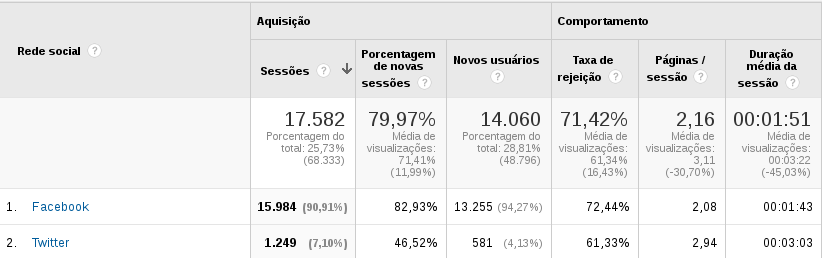
\includegraphics[scale=0.55]{./imagens/comportamento-social.png}%
	\end{center}%
	\caption{Comportamento dos usuários do Pensando O Direito advindos das redes sociais\label{fig:comportamento-redes-sociais}}%
	\fonte{Google Analytics do site \url{http://participacao.mj.gov.br/}}%
\end{figure}%

Tomando por base as informações acima observadas, é razoável recomendar que haja um trabalho de divulgação mais focado e dedicado ao twitter, sem prejuízo do trabalho realizado no Facebook. Como as ``linhas do tempo'' no Facebook não são completamente cronológicas e uma mesma postagem pode reaparecer na linha do tempo do usuário várias vezes ao dia, talvez uma única postagem diária seja suficiente para divulgação das iniciativas. Por outro lado, o Twitter possui uma linha do tempo completamente cronológica e, dessa forma, faz-se necessário um trabalho maior de postagens durante o dia, com mais de uma mensagem diária, para que se possa atingir um número maior de usuários. Outro característica distinta importante, é que o twitter trabalha com mensagens mais curtas que o Facebook, então as postagens no twitter poderiam ter uma característica mais focada numa pergunta direta com link levando à página aonde a pergunta deve ser respondida pelo usuário.

Existem ainda outros indicadores que poderiam ser avaliados na ferramenta de análise de visitantes, mas que não serão exploradas neste produto, como por exemplo os melhores horários para se postar em cada rede social para se obter a melhor conversão postagem/visitas.

\subsection{Comentários advindos das redes sociais}
Uma tendência atual de integração de sites com as redes sociais é permitir que os usuários comentem nos conteúdos do site diretamente das redes sociais, sendo estes comentários apresentados no próprio site.

Existem dois grandes problemas com esta abordagem. O primeiro deles é o confronto direto com um dos princípios expostos na introdução deste produto, que é a garantia de controle dos comentários em termos de armazenamento para fins de registro histórico. O segundo problema é que, de forma geral, os comentários realizados diretamente nas redes sociais possuem uma tendência a serem comentários de crítica esvaziada de argumentação, uma área de desabafo, e essa tendência se reduz bastante quando o usuário precisa sair da rede social, entrar em outro site, fazer seu cadastro/login para em seguida comentar, o que tende a melhorar muito a qualidade das contribuições realizadas.

Assim, recomenda-se fortemente que não haja integração que permita comentários advindos diretamente das redes sociais.

\section{Redes Sociais Federadas Públicas}
Uma integração com redes sociais que poderia agregar muito ao caráter público e coletivo das plataformas é a integração com redes sociais federadas públicas já existentes, como o Participa.br. Essa integração poderia dar-se apenas em termos de login/cadastro dos usuários, compartilhando as bases de usuários das duas plataformas, favorecendo iniciativas de intercâmbio entre ambas plataformas.

Ainda assim, como o Participa.br utiliza tecnologias muito distintas do Pensando o Direito, Noofesro naquela e Wordpress nesta, uma integração mais completa, com comentários cruzados, é algo que demandaria um esforço que pode não compensar, mas a integração de login/usuários/cadastros já é mais simples, por meio de uma API, e poderia agregar muito a ambas plataformas.

\section{SEO}
Uma característica que precisa ser melhor trabalhada nas plataformas são os recursos de \gls{seo}. Algumas técnicas e características básicas de \gls{seo} foram aplicadas ao site atual, porém existem muitas outras que não o foram e que poderiam ajudar na divulgação do Pensando O Direito e seus projetos correlatos.

Neste ponto, recomenda-se buscar um especialista em técnicas avançadas de SEO, que não contemple apenas as ferramentas de busca tradicionais, mas também que conheça e possa recomendar técnicas que melhorem o desempenho das postagens nos perfis de redes sociais, como por exemplo a utilização de \textit{hashtags}.

\section{Podcast}
Outra opção que pode ajudar na disseminação das iniciativas da SAL/MJ e do Pensando O Direito seria a criação de um Podcast sobre as iniciativas e atividades, com uma página dedicada aos podcasts.

Estes podcasts poderiam tratar de pequenos pontos relativos às diversas temáticas tratadas pela SAL/MJ com uma divulgação periódica que ajude a ``fidelizar'' os usuários.
A duração e a periodicidade depender da capacidade de produção da equipe e isso deve ser levado em conta, mas recomenda-se uma periodicidade de uma semana. Sobre a duração existem diversos modelos, desde podcasts curtos, de 10 minutos, até podcasts mais longos, de 1 hora ou mais.

Creio que o objetivo desses podcasts seriam fazer uma pequena introdução sobre os diversos assuntos tratados na SAL, projetos de Lei acompanhados, ou mesmo pontos específicos de consultas públicas em andamento, no mesmo estilo das entrevistas realizadas durante a Consulta Pública do Marco Civil da Internet. A vantagem dos podcasts é que eles são mais leves e ``portáteis'', e os usuários podem simplesmente baixá-los e ouví-los durante o dia, no trânsito, etc. Além de permitirem um debate um pouco mais aprofundado que os vídeos curtos já produzidos.


\section{Dados Pessoais}
Nesta seção iremos descrever propostas de melhorias para a aplicação de consulta pública utilizada no anteprojeto de lei de \pdp.

\subsection{Respostas a comentários}
	O primeiro ponto que demanda melhoria é a principal funcionalidade do aplicação – comentários nos trechos do ante-projeto de lei.
	Atualmente a plataforma apenas permite que os usuários opinem trechos do texto, conforme mostra a Figura \ref{fig:comentarios-dados-pessoais-hoje}.
    \begin{figure}[htb]%
        \begin{center}
            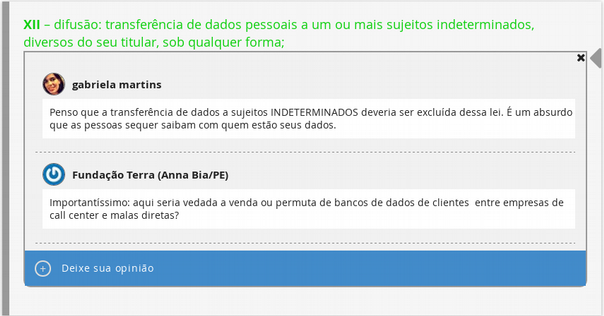
\includegraphics[scale=0.6]{./imagens/dados-pessoais-atual.png}%
        \end{center}%
        \caption{Situação atual dos comentários na ferramenta da consulta ``\pdp''\label{fig:comentarios-dados-pessoais-hoje}}%
        \fonte{Autoria Própria}%
    \end{figure}%
    
Como o objetivo é que haja um debate, é fundamental permitir que os usuários possam responder a comentários feitos, e que isso seja apresentado na forma de comentários agrupados e aninhados, permitindo um melhor desenvolvidomento do debate propriamente dito. Assim, propõe-se que seja implementado o recurso de resposta a comentários, conforme pode ser observado na Figura \ref{fig:comentarios-dados-pessoais-proposta}.
    \begin{figure}[htb]%
        \begin{center}
            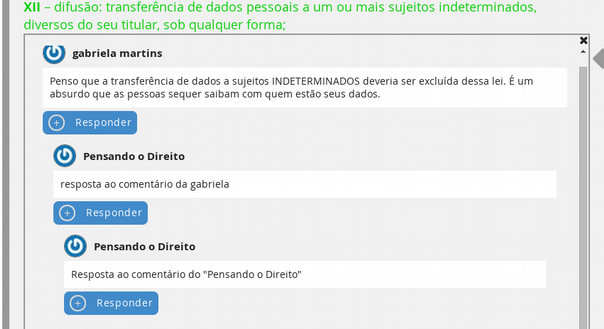
\includegraphics[scale=0.6]{./imagens/dados-pessoais-comment-novo.png}%
        \end{center}%
        \caption{Proposta de modificação com ``Respostas'' \label{fig:comentarios-dados-pessoais-proposta}}%
        \fonte{Autoria Própria}%
    \end{figure}%
    
\subsection{Implementação}
Para se chegar a tal resultado, será necessário modificar o plugin “wp-side-comments” e também realizar modificações no tema do wordpress utilizado na aplicação (“dadospessoais-tema”).
	Com relação ao plugin ``wp-side-comments'', a implementação passará por algumas modificações pequenas nos arquivos ``wp-side-comments.php'' e ``wp-side-comments.js'' e por grandes modificações no arquivo ``side-comments.js'', plugin javascript independente que implementa a funcionalidade de ``comentários laterais''.
	Relativo ao tema “dadospessoais-tema”, será necessário modificar o arquivo ``dadospessoais.js'' para implementar o template e alguma lógica para as respostas, além do desenvolvimento de regras de estilo CSS.
	
\subsection{Concordar / Discordar}
Outra possibilidade a ser ponderada é a adição de botões ``concordar'' e ``discordar'', permitindo que os usuários interajam com os comentários/respostas de outros usuários pode meio de endossos ou reprovações de opiniões já expressas.
	Deve-se ponderar a utilização deste recurso pois, por um lado, ele pode desestimular a participação dos usuários por meio da expressão escrita de suas opiniões, restringindo-se a ``votar''. Por outro lado, este seria um recurso de grande valia para a sistematização das contribuições feitas na consulta.
	Como forma de tentar estimular colaborações textuais, reduzindo o efeito negativo do recurso ``voto'', após o usuário votar poderia ser apresentado a ele um ``box'' convidando-o a expor os motivos pelos quais ele concorda ou discorda – a depender do voto dado; daquele comentário. Assim, uma ação simples e rápida (voto) pode vir a ser convertida num texto que complemente uma opinião anteriormente exposta ou num texto que exponha pontos de fragilidade de um argumento.
	Este recurso poderia ser desenvolvido enquanto uma \textit{feature} do plugin ``wp-side-comments'' de forma que esta feature possa ser ativada ou desativada, permitindo assim sua utilização quando for considerada conveniente.
	
\subsection{Redes Sociais}
Outro recurso que pode contribuir para o debate público, caso venha a ser implementado, é permitir que os usuários compartilhem trechos específicos do texto em debate nas redes sociais, ou que ao inserir um comentário na aplicação que este comentário seja automaticamente distribuído na rede social com o link de referência de volta para o comentário. Desta forma, pode-se potencializar o debate e atrair novas pessoas por meio da atuação dos próprios usuários.

\subsection{Implementação}
	A implementação deste novo recurso também passará por modificações no plugin ``wp-side-comments'' e no tema ``dadospessoais-tema''. Será preciso implementar um link permanente (permalink) para cada trecho de texto e/ou comentário, de forma que este permalink possa ser compartilhado nas redes sociais, dando acesso direto ao trecho ou comentário.
\section{Marco Civil da Internet}
Com relação à ferramenta de consulta da Regulamentação do \mc, ela se apresenta como uma ferramenta bem mais completa que a anterior. Alguns ajustes visuais poderiam melhorar sua usabilidade – mas estes não são o foco do presente trabalho. Em termos de recursos, vislumbram-se duas possíveis melhorias que poderiam aumentar a participação.

\subsection{Comentários em ``sanfona''}
A primeira delas seria mostrar os comentários das pautas na página de listagem de pautas, sem que fosse necessário o usuário mudar de página. Na Figura \ref{fig:pautas-mcivil-hj} apresenta-se a página com a listagem de todas as pautas correntes. Nela podemos observar que o número de comentários de cada pauta está apresentado, porém para ver o comentário é preciso navegar até a página da pauta. Seria interessante que a visualização dos comentários (e a adição de novos) pudesse ser realizada na própria página de listagem de pauta, num fluxo similar ao fluxo do plugin wp-side-comments utilizado na consulta do anteprojeto de lei de proteção de dados pessoais.
    \begin{figure}[htb]%
        \begin{center}
            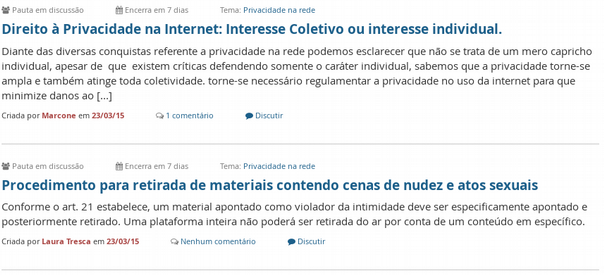
\includegraphics[scale=0.7]{./imagens/mcivil-atual-listagem.png}%
        \end{center}%
        \caption{Versão autal da listagem de pautas na consulta do \mc \label{fig:pautas-mcivil-hj}}%
        \fonte{Autoria Própria}%
    \end{figure}%
    
\subsection{Concordar / Discordar}
A segunda modificação seria a implementação do recurso ``concordar/discordar'' na própria pauta, não apenas nos comentários da mesma como é hoje, conforme pode ser observado na Figura \ref{fig:pauta-espec-mcivil}. De maneira análoga ao que foi proposto anteriormente, seria interessante após o voto de ``acordo'' ou ``desacordo'' convidar o usuário a explicar os motivos pelos quais ele concordou ou discordou do comentário e/ou da pauta.
    \begin{figure}[htb]%
        \begin{center}
            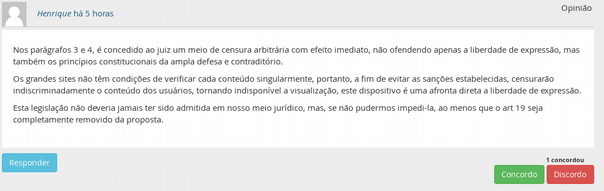
\includegraphics[scale=0.7]{./imagens/mcivil-comentario-pauta.png}%
        \end{center}%
        \caption{Comentário de uma Pauta específica \label{fig:pauta-espec-mcivil}}%
        \fonte{Autoria Própria}%
    \end{figure}%

\subsection{Redes Sociais}
	Se faz também necessária a implementação de recurso de compartilhamento de pautas/comentários/temas nas redes sociais, para que se possa atingir um público maior e aumentar as chances de colaboração. Este compartilhamento pode-se dar em alguns instantes distintos.
	
	O primeiro deles é simplesmente compartilhar uma pauta inserida por outrém. Este recurso está disponível, mas apenas dentro da página da pauta, quando ele poderia estar disponível na página de listagem de pautas também. Além disso, ele precisa ficar mais evidente. Conforme pode-se observar nas Figuras \ref{fig:pauta-espec-mcivil-share-comentario-fechado} e \ref{fig:pauta-espec-mcivil-share-comentario-ativo}, não está claro que existe a possibilidade de compartilhamento da pauta enquanto um recurso de rede social. Talvez a simples mudança na simbologia utilizada seja o suficiente neste caso, mas a mudança do posicionamento, alinhando o botão de compartilhamento com o título da pauta também pode ajudar.
    \begin{figure}[htb]%
        \begin{center}
            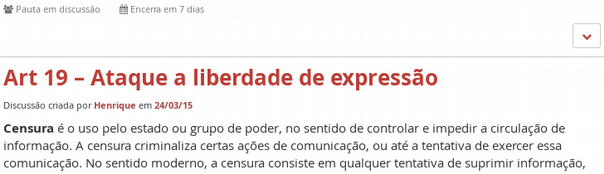
\includegraphics[scale=0.7]{./imagens/mcivil-social-share-01.png}%
        \end{center}%
        \caption{Página de uma pauta específica – Botão de compartilhamento quase escondido \label{fig:pauta-espec-mcivil-share-comentario-fechado}}%
        \fonte{Autoria Própria}%
    \end{figure}%
    \begin{figure}[htb]%
        \begin{center}
            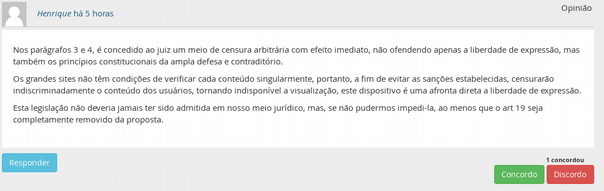
\includegraphics[scale=0.7]{./imagens/mcivil-comentario-pauta.png}%
        \end{center}%
        \caption{Página de pauta específica - Botão de compartilhamento ativo \label{fig:pauta-espec-mcivil-share-comentario-ativo}}%
        \fonte{Autoria Própria}%
    \end{figure}%
	Outro momento em que a opção de compartilhamento deveria ser apresentada aos usuários é ao inserir uma nova pauta, publicando-a no sistema e nas redes sociais simultâneamente.
	
	Por fim, ao adicionar um novo comentário (ou voto) numa pauta também deveria ser apresentada a opção de compartilhar o comentário (ou voto) nas redes sociais do usuário.

	Todas estas modificações seriam feitas no plugin “delibera” atualmente em uso na referida consulta.

\subsection{Pautas em destaque}
Para tentar fomentar ainda mais os debates, pode ser útil oferecer aos usuários a possibilidade de ver quais são as pautas mais debatidas, e talvez mais ``polêmicas''. Para isso existem duas possibilidades.

	A primeira delas é permitir reordenar as pautas pelo número de comentários (ou votos).

	A segunda delas é a utilização de ``marcadores'' de destaque. Pode-se pensar em ícones como o apresentado na Figura \ref{fig:mcivil-icone-pauta-destaque}, dentre outros.
	    \begin{figure}[htb]%
        \begin{center}
            
\includegraphics[scale=0.7]{./imagens/hot-topic.png}%
        \end{center}%
        \caption{Ícone de marcação de pauta em destaque \label{fig:mcivil-icone-pauta-destaque}}%
        \fonte{Autoria Própria}%
    \end{figure}%

\subsection{Ordenamento de pautas}
Visando facilitar a colaboração de usuários mais engajados, além de auxiliar em sistematizações, seria importante permitir também a ordenação das pautas por diversos critérios, sendo os principais:
\begin{itemize}
\item Quantidade de comentários;
\item Data de postagem;
\item Últimos comentários;
\item Quantidade de votos "concordo"; e
\item Quantidade de votos "discordo".
\end{itemize}

Desta forma os usuários mais ativos na plataforma podem encontrar de forma mais fácil os itens que possuem mais atividade, ou mais atividades recentes, sem precisar passar por todas as postagens.

O mesmo vale para a equipe que ficará responsável pela organização/sistematização da consulta, que poderá, ao longo do processo, acompanhar o desenvolvimento da consulta e, ao final, realizar destaques de forma simplificada.
\section{Métodologia de Trabalho}
Para o bom desenrolar das atividades de desenvolvimento, é de fundamental importância o estebelecimento de um método de trabalho claro para que todos \textit{stakeholders} consigam constribuir sem \textit{overheads} de compatibilização de trabalhos e/ou conflitos.

Assim, faz-se aqui uma proposta de método de trabalho baseada em princípios das metodologias ágeis.
\subsection{Estratégia de versionamento}
A estratégia de versionamento proposta é uma variação do conhecido \textit{workflow} \textit{gitFlow}%
\footnote{\textit{Git Flow: a successful branching model}, modelo de versionamento proposto por Vincent Driessen, da nvie (\url{http://nvie.com/}), em Janeiro de 2010 e que faz muito sucesso. \url{http://nvie.com/posts/a-successful-git-branching-model/} - Acessado em 01/03/2015}, que pode ser observado na Figura \ref{fig:gitflow}.

    \begin{figure}[htb]%
        \begin{center}
            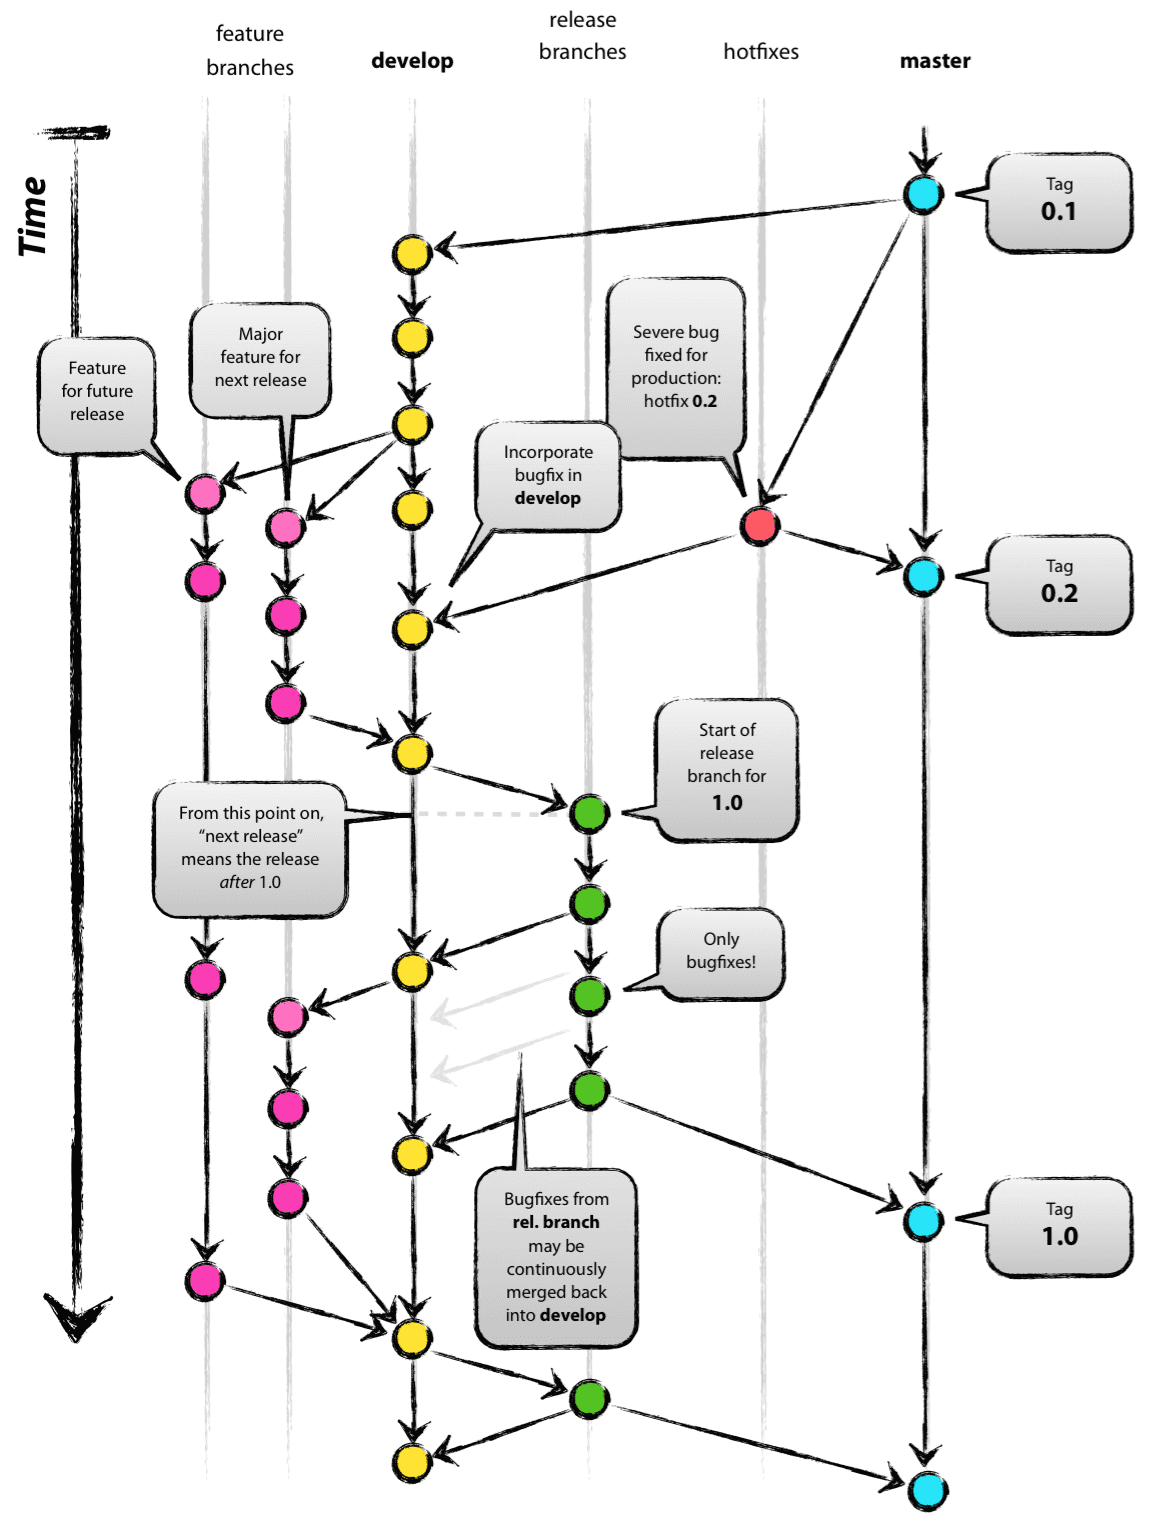
\includegraphics[scale=0.23]{./imagens/gitflow.png}%
        \end{center}%
        \caption{Diagrama da estratégia conhecida como GitFlow \label{fig:gitflow}}%
        \fonte{Vincent Driessen - \url{http://nvie.com/posts/a-successful-git-branching-model/} - Acessado em 01/03/2015}%
    \end{figure}%
    
O \textit{GitFlow} propõe que todos os desenvolvedores atuem diretamente no repositório principal do projeto, sendo que o trabalho é desenvolvido baseado em \textit{features} (recursos) e que o desenvolvimento de cada \textit{feature} é realizado num \textit{branch} criado especificamente para aquela feature. A integração das features é realizada num \textit{branch} chamado ``desenvolvimento'' e, de tempos em tempos, são fecha-se uma versão para publicação, que após integrada e testada é enviada ao \textit{branch} ``\textit{master}'', que conterá as versões estáveis do projeto, marcadas por meio de \textit{tags}.

Para se adequar à realidade da atual equipe de desenvolvimento da \gls{sal}, cada desenvolvedor deve realizar um \textit{fork} (bifurcação) do projeto dentro de seu próprio usuário do github e, em seguida, trabalhar utilizando o modelo do \textit{GitFlow} dentro de seu próprio \textit{fork}, utilizando o modelo de \textit{branches} proposto. Após a finalização de alguma \textit{feature}, a pessoa deve realizar um \textit{Pull-Request} de seu repositório para o repositório principal do projeto, para que este \textit{Pull-Request} possa ser avaliado pelo gestor do projeto e integrado ao repositório principal.

Outra modificação, necessária em função do legado já existente de trabalho do projeto, é que as integrações das \textit{features} ocorrerão no \textit{branch} ``master'', e não no ``desenvolvimento'', e as versões estáveis serão consolidadas no \textit{branch} ``stable''. Isso tanto no repositório principal quanto nos repositórios dos desenvolvedores.

Com isso, os desenvolvedores devem integrar suas features desenvolvidas em \textit{branches} no seu próprio repositório ``master'', realizar o \textit{Pull-request} para o repositório ``master'' do projeto principal e, no projeto principal, o \textit{branch} ``master'' será integrado ao ``stable'' com periodicidade a ser definida. A sequência abaixo resume este fluxo de trabalho, muito similar ao ``\textit{Forking Workflow}''\footnote{``\textit{Forking Workflow}'' - \url{https://www.atlassian.com/git/tutorials/comparing-workflows/forking-workflow} - Acessado em 12/03/2015}.
\newpage
\subsubsection{Passo a passo do \textit{workflow} de versionamento proposto}
Passo 1 - O gestor do projeto cria o repositório principal do projeto no ``servidor central'' (github)\footnote{No caso do presente projeto o serviço GitHub (\url{http://github.com}) será utilizado como servidor central dos repositórios de código do projeto}:
    \begin{figure}[htb]%
        \begin{center}
            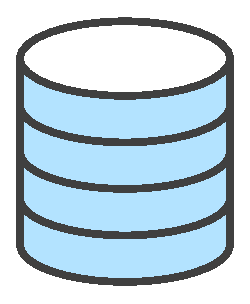
\includegraphics[scale=0.2]{./imagens/forkflow.eps}%
        \end{center}%
        \caption{Workflow de versionamento - passo 01 \label{fig:forkflow01}}%
        \fonte{Atlassian - Comparing Workflows - Acessado em 12/03/2015}%
    \end{figure}%

Passo 2 - Cada integrante da equipe de desenvolvimento cria seu próprio \textit{fork} no github:
    \begin{figure}[htb]%
        \begin{center}
            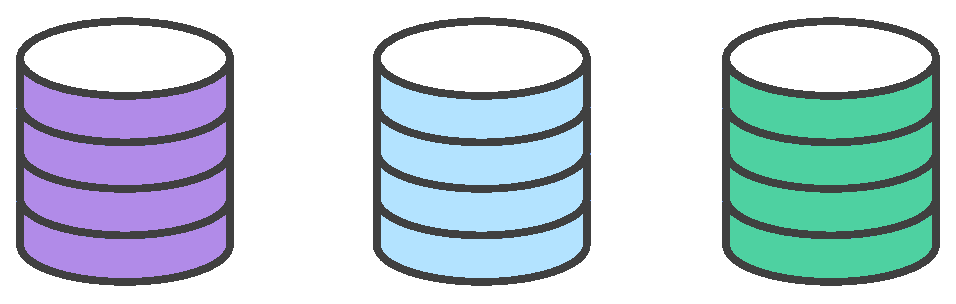
\includegraphics[scale=0.2]{./imagens/forkflow2.eps}%
        \end{center}%
        \caption{Workflow de versionamento - passo 02 \label{fig:forkflow02}}%
        \fonte{Atlassian - Comparing Workflows - Acessado em 12/03/2015}%
    \end{figure}%
    
Passo 3 - Cada integrante da equipe clona seu \textit{fork} em sua máquina local:
    \begin{figure}[htb]%
        \begin{center}
            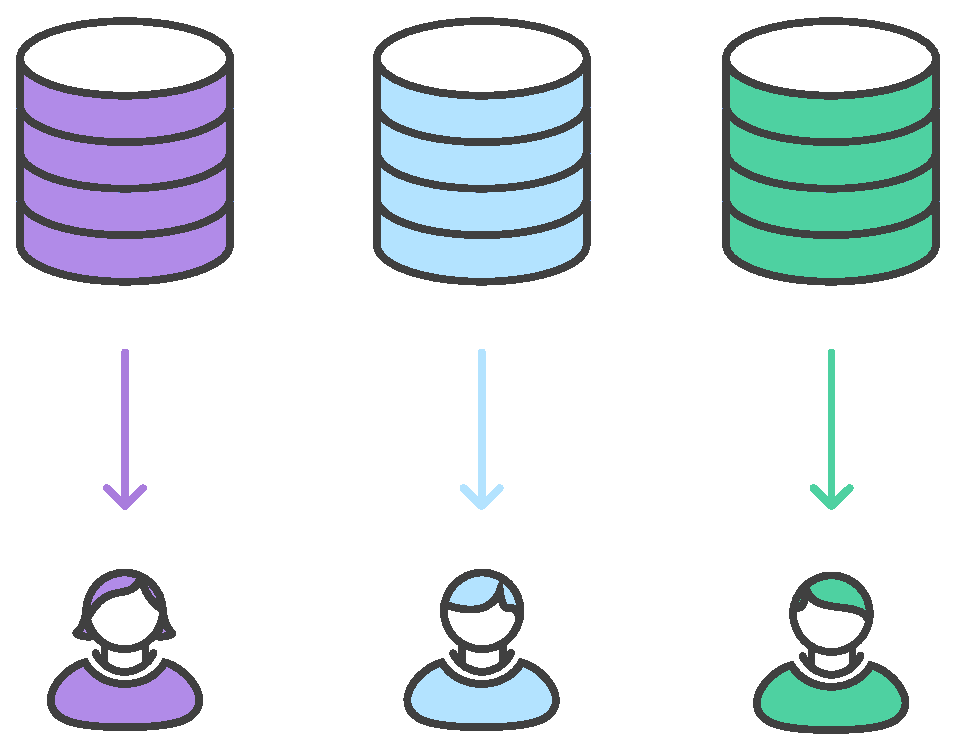
\includegraphics[scale=0.2]{./imagens/forkflow3.eps}%
        \end{center}%
        \caption{Workflow de versionamento - passo 03 \label{fig:forkflow03}}%
        \fonte{Atlassian - Comparing Workflows - Acessado em 12/03/2015}%
    \end{figure}%
\newpage
Passo 4 - Cada integrante da equipe desenvolve suas \textit{features} em \textit{branches} locais:
    \begin{figure}[htb]%
        \begin{center}
            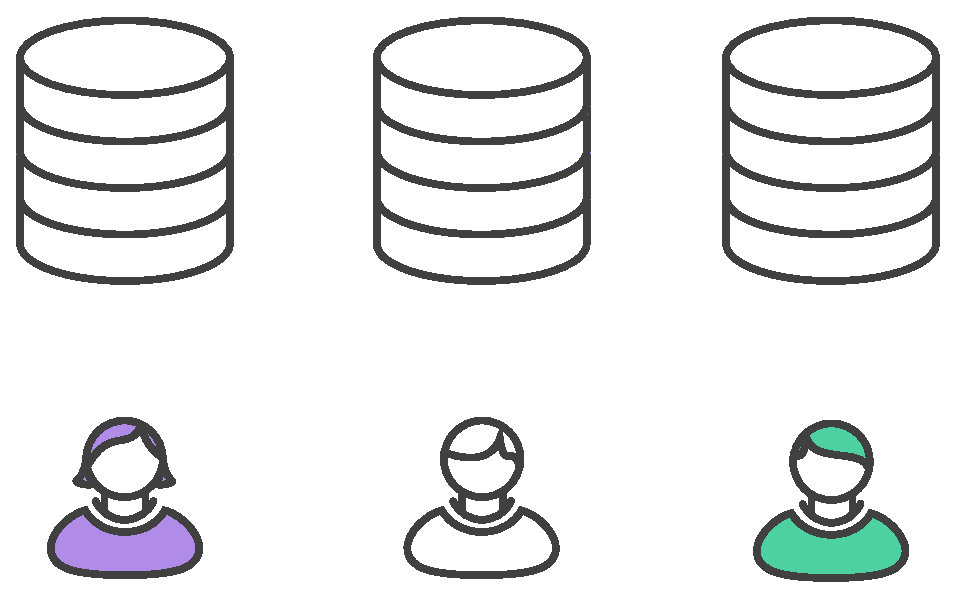
\includegraphics[scale=0.2]{./imagens/forkflow4.eps}%
        \end{center}%
        \caption{Workflow de versionamento - passo 04 \label{fig:forkflow04}}%
        \fonte{Atlassian - Comparing Workflows - Acessado em 12/03/2015}%
    \end{figure}%
    
Passo 5 - Após finalizada a \textit{feature}, o \textit{branch} da \textit{feature} é enviado para o repositório (\textit{fork}) do usuário no github. Caso haja mais de uma pessoa trabalhando na mesma \textit{feature}, recomenda-se que o \textit{branch} da \textit{feature} seja publicado constantemente ao \textit{fork} do usuário de forma que outro desenvolvedor possa utilizar as modificações feitas - realizando um \textit{pull} daquele \textit{branch} para seu repositório.
    \begin{figure}[htb]%
        \begin{center}
            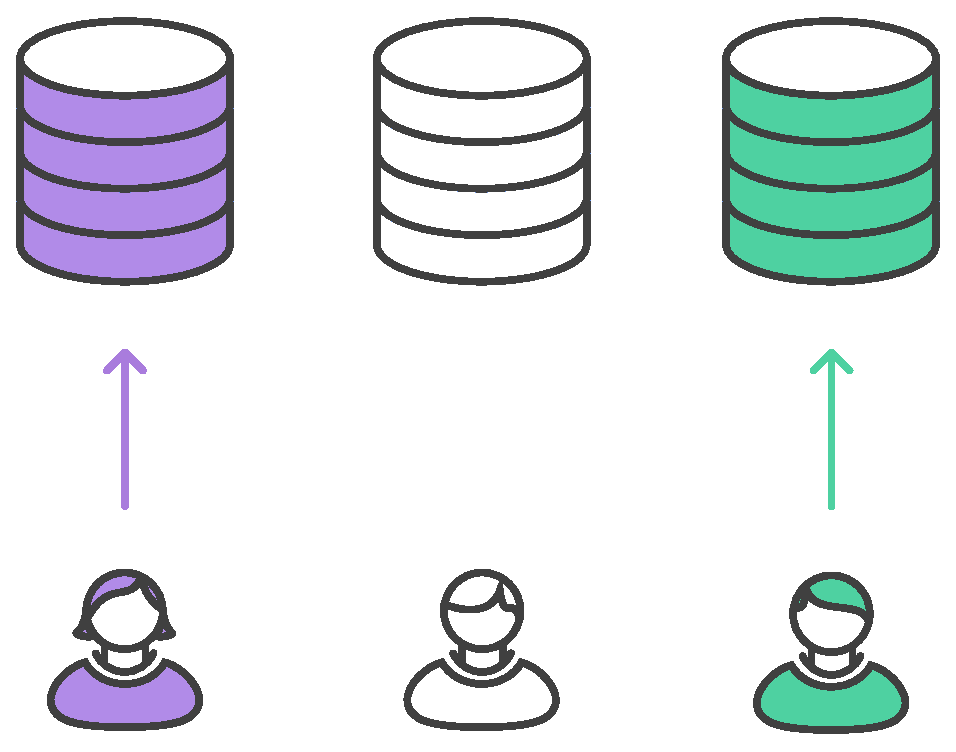
\includegraphics[scale=0.2]{./imagens/forkflow5.eps}%
        \end{center}%
        \caption{Workflow de versionamento - passo 05 \label{fig:forkflow05}}%
        \fonte{Atlassian - Comparing Workflows - Acessado em 12/03/2015}%
    \end{figure}%
\newpage
Passo 6 - Cada responsável por uma \textit{feature} realiza um \textit{Pull-Request} do \textit{branch} de sua \textit{feature} em seu \textit{fork} para o \textit{branch} ``master'' do repositório principal do projeto. Com os \textit{Pull-Requests} o gestor do projeto, no papel de integrador, verifica cada \textit{Pull-Request}, aceita (ou não) o \textit{Pull Request} e integra, uma a uma, as \textit{features} no repositório branch ``master'' de seu repositório local. Neste momento, cada \textit{Pull-Request} representará uma nova \textit{feature} (ou a resolução de algum \textit{bug}/\textit{issue}), e a cada integração deve-se realizar a validação da mesma.
    \begin{figure}[htb]%
        \begin{center}
            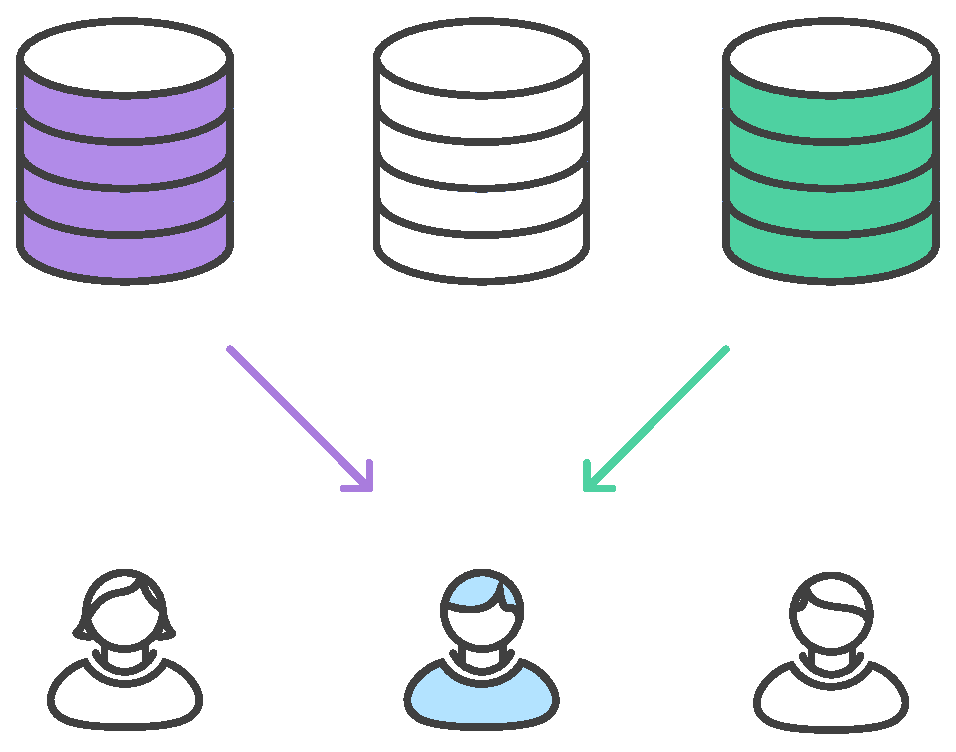
\includegraphics[scale=0.2]{./imagens/forkflow6.eps}%
        \end{center}%
        \caption{Workflow de versionamento - passo 06 \label{fig:forkflow06}}%
        \fonte{Autoria Própria}%
    \end{figure}%

Passo 7 - Após as integrações serem realizadas, o gestor deve enviar o \textit{branch} ``master'' de seu repositório local para o repositório principal do projeto.
    \begin{figure}[htb]%
        \begin{center}
            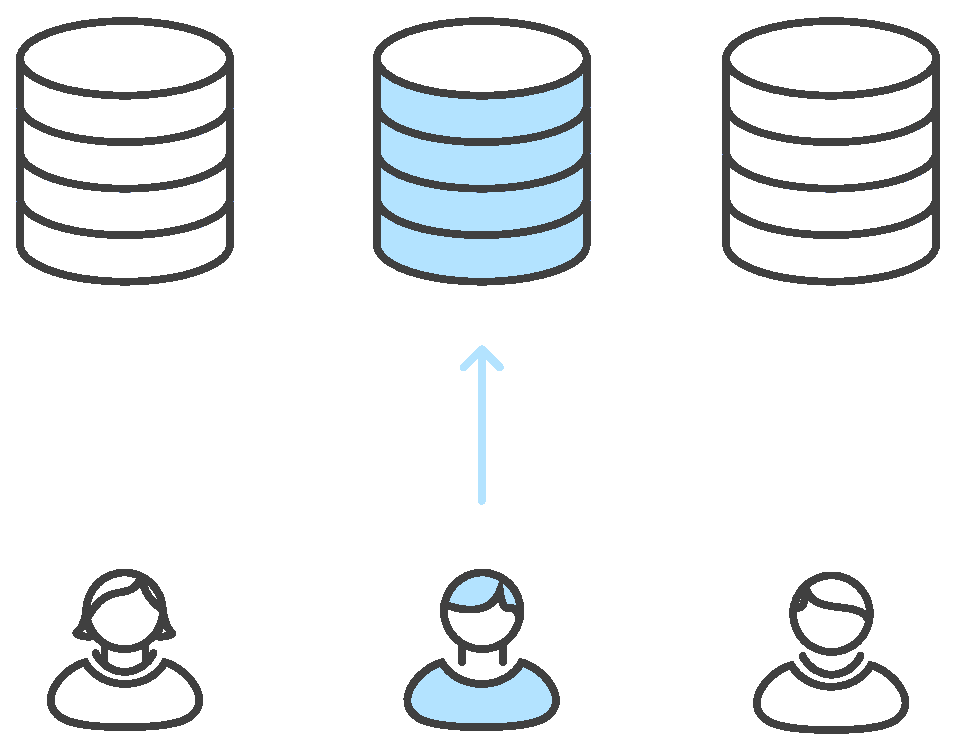
\includegraphics[scale=0.2]{./imagens/forkflow7.eps}%
        \end{center}%
        \caption{Workflow de versionamento - passo 07 \label{fig:forkflow07}}%
        \fonte{Autoria Própria}%
    \end{figure}%
\newpage
Passo 8 - Após a integração das \textit{features} ao repositório principal, todas pessoas que integram a equipe de desenvolvimento sincronizam novamente o \textit{branch} ``master'' de seus \textit{forks} com o \textit{branch} ``master'' do repositório principal.
    \begin{figure}[htb]%
        \begin{center}
            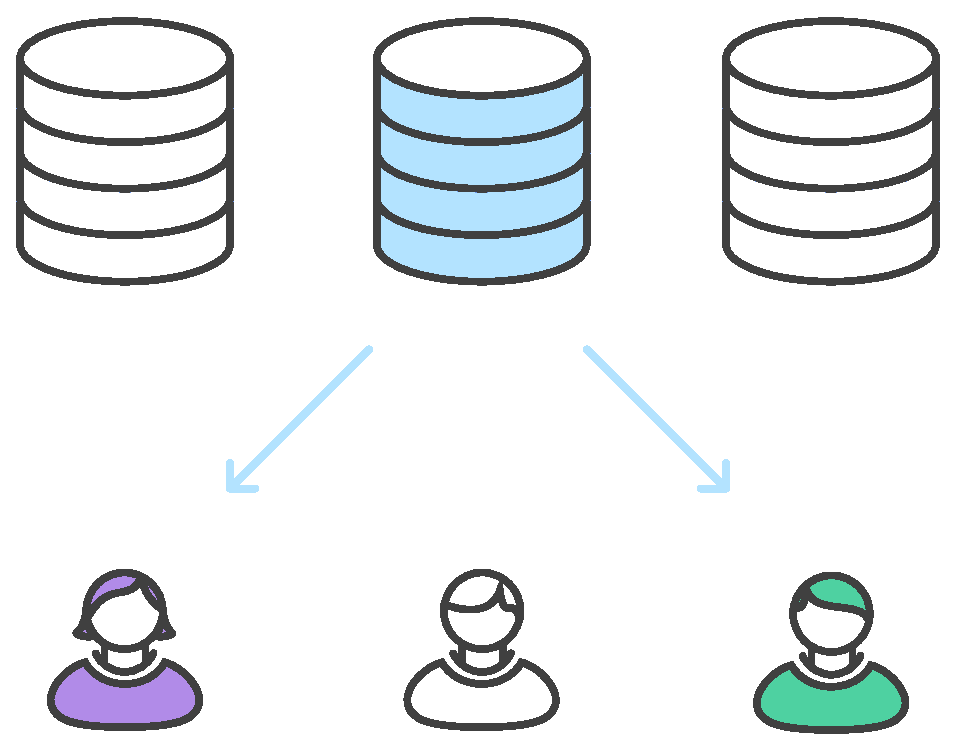
\includegraphics[scale=0.2]{./imagens/forkflow8.eps}%
        \end{center}%
        \caption{Workflow de versionamento - passo 08 \label{fig:forkflow08}}%
        \fonte{Atlassian - Comparing Workflows - Acessado em 12/03/2015}%
    \end{figure}%

Passo 9 - Periodicamente\footnote{A periodicidade depende do modelo de trabalho adotado, que não está definido neste processo de versionamento de código.}, após as integrações realizadas, o gestor define um \textit{release} e marca o repositório com uma \textit{tag} que defina tal \textit{release}, que em seguida será implementado no site em produção\footnote{O processo de implantação de novas versões em produção deve ser definido em outro documento.}.
    \begin{figure}[htb]%
        \begin{center}
            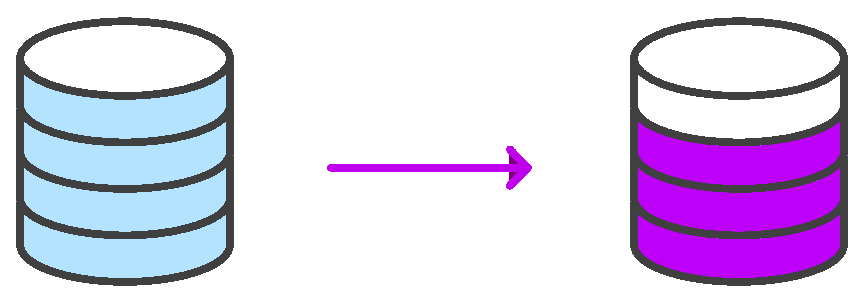
\includegraphics[scale=0.2]{./imagens/forkflow9.eps}%
        \end{center}%
        \caption{Workflow de versionamento - passo 09 \label{fig:forkflow09}}%
        \fonte{Atlassian - Comparing Workflows - Acessado em 12/03/2015}%
    \end{figure}%


% ---
% Conclusão
\chapter{Conclusão}
Este documento apresenta a necessidade e a importância do processo de sistematização de constribuições realizadas em ambientes de colaboração, em especial quando se trata da relação entre sociedade civil e governos. Esta ainda é uma área completamente em aberto e que demanda muitas experimentações e estudos.

Existem diversas formas de a sociedade civil trabalhar em parceria com o governo, sendo uma delas a colaboração na construção das ferramentas de participação social. Para tanto, é fundamental que o processo de desenvolvimento de ferramentas esteja bem documentado e seja orientado a colaborações de terceiros. Assim, apresentamos na seção \ref{sec:metodologia-agil} uma proposta de Metodologia que visa contemplar colaboradores externos e pontuais.

Além disso, como parte do processo de aprendizado e experimentação em participação social, propõe-se aqui a implementação da ferramenta \textit{Hypotes.is} para ser utilizada na sistematização das contribuições realizadas na consulta pública do \mc e do \pdp. Posteriormente se faz necessária uma avaliação de como se deu a utilização desta ferramenta neste processo.

Por fim, são apresentadas também algumas alternativas de ferramentas e tecnologias que poderiam ser utilizadas em conjunto com o \textit{Hypotes.is} para automatizar o processo de avaliação e sistematização das contribuições.

% ---

% ----------------------------------------------------------
% ELEMENTOS PÓS-TEXTUAIS
% ----------------------------------------------------------
\postextual

% ----------------------------------------------------------
% Referências bibliográficas
% ----------------------------------------------------------
\bibliography{referencias}


% ---
% inserindo listas (tabelas, ilustrações, etc.)
% inserir lista de ilustrações
\pdfbookmark[0]{\listfigurename}{lof}
\listoffigures
\cleardoublepage
% ---

% ---
% inserir lista de tabelas
% ---
%\pdfbookmark[0]{\listtablename}{lot}
%\listoftables*
%\cleardoublepage
% ---



% ---
% inserir lista de abreviaturas e siglas


% ----------------------------------------------------------
% Glossário
% ----------------------------------------------------------
%
% Consulte o manual da classe abntex2 para orientações sobre o glossário.
%
%\glossary

% ----------------------------------------------------------
% Apêndices
% ----------------------------------------------------------

% ---
% Inicia os apêndices
% ---
%\begin{apendicesenv}

% Imprime uma página indicando o início dos apêndices
%\partapendices

% ----------------------------------------------------------
%\chapter{Primeiro apêndice}
% ----------------------------------------------------------

%\end{apendicesenv}
% ---

% ----------------------------------------------------------
% Anexos
% ----------------------------------------------------------

% ---
% Inicia os anexos
% ---
%\begin{anexosenv}

% Imprime uma página indicando o início dos anexos
%\partanexos

% ---
%\chapter{Primeiro Anexo}

%\end{anexosenv}

%---------------------------------------------------------------------
% INDICE REMISSIVO
%---------------------------------------------------------------------
%
%\phantompart
%
%\printindex

%---------------------------------------------------------------------
% Formulário de Identificação (opcional)
%---------------------------------------------------------------------
%\chapter*[Formulário de Identificação]{Formulário de Identificação}
%\addcontentsline{toc}{chapter}{Exemplo de Formulário de Identificação}
%\label{formulado-identificacao}
%
%%Exemplo de Formulário de Identificação, compatível com o Anexo A (informativo) da ABNT NBR 10719:2011. Este formulário não é um anexo. Conforme definido na norma, ele é o último elemento pós-textual e opcional do relatório.
%
%\bigskip
%
%\begin{tabular}{|p{9cm}|p{5cm}|}
%\hline
%\multicolumn{2}{|c|}{\textbf{\large Dados do Relatório Técnico}}\\
%\hline
%\multirow{4}{9cm}{{Relatório contendo avaliação e propostas de melhorias técnicas para ferramentas e aplicações de consulta pública, incluindo plugins}}& Classificação de segurança\\
%                    & \\
%                   \cline{2-2}
%                   & No.\\
%                    & 1 \\
%				
%\hline
%Relatório Técnico & 13/03/2015\\
%\hline
%{Projeto Democratização de Informações no Processo de Elaboração Normativa} & No. BRA/07/004\\
%\hline
%\multicolumn{2}{|l|}{Diego Rabatone Oliveira} \\
%\hline
%\multicolumn{2}{|l|}{Secretaria de Assuntos Legislativos do Ministério da Justiça (SAL/MJ)} \\
%\hline
%\multicolumn{2}{|l|}{Programa das Nações Unidas para o Desenvolvimento (PNUD)} \\
%\hline
%\multicolumn{2}{|l|}{\multirow{1}{0.9\textwidth}{Este produto objetiva realizar uma avaliação técnica das ferramentas e aplicações de consulta pública do projeto “Pensando o Direito”, do Ministério da Justiça. Além da avaliação serão também propostas melhorias dos recursos já existentes, tendo como objetivo secundário a publicização de tais melhorias enquanto ferramentas livres que possam ser reutilizadas pela sociedade. Para o desenvolvimento deste trabalho foi utilizada metodologia de desenvolvimento ágil, com definição de tarefas a serem realizada e sprints para a realização das mesmas. Resulta ainda deste trabalho uma recomendação de método de trabalho da equipe de desenvolvimento.}}\\[5cm]
%\hline
%\multicolumn{2}{|l|}{\multirow{1}{0.9\textwidth}{Palavras-Chaves: Wordpress, \mc, \pdp, Métodos Ágeis}}\\[0.7cm]
%\hline
%\multicolumn{2}{|l|}{
%1$^a$Edição \hfill \pageref{LastPage} páginas \hfill Volume 1 \hfill Nº de classificação \phantom{XXXX}} \\
%\hline
%\multicolumn{2}{|l|}{ISSN \phantom{XXXX}\hfill Tiragem \phantom{XXXX}} \\
%\hline
%%\multicolumn{2}{|l|}{Distribuidor} \\
%%\hline
%%\multicolumn{2}{|l|}{Observações/notas}\\[3cm]
%%\hline
%\end{tabular}
%
\end{document}